\documentclass[a4paper, 12pt]{article}

\usepackage{hyperref}
\usepackage[warn]{mathtext}
\usepackage[utf8]{inputenc}
\usepackage[T2A]{fontenc}
\usepackage[english,russian]{babel}
\usepackage{multirow}
\usepackage{float}
\restylefloat{table}
\usepackage{amsmath,amsfonts,amssymb,amsthm,mathtools}
\usepackage{indentfirst}
\DeclareSymbolFont{T2Aletters}{T2A}{cmr}{m}{it}
\usepackage{ gensymb }
\mathtoolsset{showonlyrefs=true}
\usepackage{euscript}
\usepackage{mathrsfs}
\usepackage[left=2cm,right=2cm,top=2cm,bottom=2cm]{geometry}
\usepackage{graphicx}
\usepackage{wrapfig}
\usepackage[rgb]{xcolor}
\hypersetup{
colorlinks=true,
urlcolor=blue
}
\usepackage{tikz}

\title{Лабораторная работа}
\author{Гисич Арсений Б03-101}
\date{2023}

\begin{document}

	\begin{center}
		{\large МОСКОВСКИЙ ФИЗИКО-ТЕХНИЧЕСКИЙ ИНСТИТУТ (НАЦИОНАЛЬНЫЙ ИССЛЕДОВАТЕЛЬСКИЙ УНИВЕРСИТЕТ)}
	\end{center}
	\vspace{5 cm}
	{\Large
		\begin{center}
			{\bf Лабораторная работа 5.1.2}\\[0.2 cm]
			Исследование эффекта Комптона
		\end{center}
	}
	\vspace{4 cm}
	\begin{flushright}
		{\Large Выполнили: \\
			\vspace{0.2 cm}
			Гисич Арсений \\
            Вазюля Василиса \\ 
			\vspace{0.2 cm}
			Б03-101 \\}
	\end{flushright}
	\vspace{8 cm}
	\begin{center}
		Долгопрудный\\[0.1 cm]
		2023
	\end{center}
\thispagestyle{empty}

\section{Аннотация}

В данной работе с помощью сцинтилляционного спектрометра исследуется энергетический спектр $\gamma$-квантов, рассеянных на графите. Определяется энергия рассеянных $\gamma$ -квантов в зависимости от угла рассеяния, а также энергия покоя частиц, на которых происходит комптоновское рассеяние.

\section{Теоретические сведения}

Рассеяние $\gamma$-лучей в веществе относится к числу явлений, в которых особенно ясно проявляется двойственная природа излучения. Волновая теория, хорошо объясняющая рассеяние длинноволнового излучения, испытывает трудности при описании рассеяния рентгеновских и $\gamma$-лучей. Эта теория, в частности, не может объяснить, почему в составе рассеянного излучения, измеренного Комптоном, кроме исходной волны с частотой $\omega_{0}$ появляется дополнительная длинноволновая компонента, отсутствующая в спектре первичного излучения.

Появление этой компоненты легко объяснимо, если считать, что $\gamma$-излучение представляет собой поток квантов (фотонов), имеющих энергию $\hbar \omega$ и импульс $p=\hbar \omega / c .$ Эффект Комптона --- увеличение длины волны рассеянного излучения по сравнению с падающим --- интерпретируется как результат упругого соударения двух частиц: $\gamma$-кванта (фотона) и свободного электрона.

Рассмотрим элементарную теорию эффекта Комптона. Пусть электрон до соударения покоился (его энергия равна энергии покоя $m c^{2}$ ), a $\gamma$-квант имел начальную энергию $\hbar \omega_{0}$ и импульс $\hbar \omega_{0} / c .$ После соударения электрон приобретает энергию $\gamma m c^{2}$ и импульс $\gamma m v,$ где $\gamma = \left(1-\beta^{2}\right)^{-1 / 2}, \beta=v / c,$ a $\gamma$-квант рассеивается на некоторый угол $\theta$ по отношению к первоначальному направлению движения. Энергия и импульс $\gamma$-кванта становятся соответственно равным и $\hbar \omega_{1}$ и $\hbar \omega_{1} / c$ (рис. 1). Запишем для рассматриваемого процесса законы сохранения энергии и импульса:
$$
\begin{array}{c}
m c^{2}+\hbar \omega_{0}=\gamma m c^{2}+\hbar \omega_{1} \\
\frac{\hbar \omega_{0}}{c}=\gamma m v \cos \varphi+\frac{\hbar \omega_{1}}{c} \cos \theta \\
\gamma m v \sin \varphi=\frac{\hbar \omega_{1}}{c} \sin \theta
\end{array}
$$
Решая совместно эти уравнения и переходя от частот $\omega_{0}$ и $\omega_{1}$ к длинам волн $\lambda_{0}$ и $\lambda_{1},$ нетрудно получить, что изменение длины волны рассеянного излучения равно
\begin{equation}
\Delta \lambda=\lambda_{1}-\lambda_{0}=\frac{h}{m c}(1-\cos \theta)=\Lambda_{\mathrm{K}}(1-\cos \theta)
\end{equation}
где $\lambda_{0}$ и $\lambda_{1}$ --- длины волн $\gamma$-кванта до и после рассеяния, а величина
$$
\Lambda_{\mathrm{K}}=\frac{h}{m c}=2,42 \cdot 10^{-10} \mathrm{cm}
$$

Основной целью данной работы является проверка соотношения
(1). Применительно к условиям нашего опыта формулу
(1) следует преобразовать от длин волн к энергии $\gamma$-квантов. Как нетрудно показать, соответствующее выражение имеет вид
\begin{equation}
\frac{1}{\varepsilon(\theta)}-\frac{1}{\varepsilon_{0}}=1-\cos \theta
\end{equation}
Здесь $\varepsilon_{0}=E_{0} /\left(m c^{2}\right)-$ выраженная в единицах $m c^{2}$ энергия $\gamma$-квантов, падающих на рассеиватель, $\varepsilon(\theta)$ --- выраженная в тех же единицах энергия квантов, испытавших комптоновское рассеяние на угол $\theta$, $m$ --- масса электрона.

\section{Методика измерений}

Блок-схема установки изображена на рис. $3 .$ Источником излучения 1 служит $\mathrm{Cs}^{137}$, испускающий $\gamma$-лучи с энергией 662 кэВ. Он помещен в толстостенный свинцовый контейнер с коллиматором. Сформированный коллиматором узкий пучок $\gamma$-квантов попадает на графитовую мишень 2 (цилиндр диаметром 40 мм и высотой 100 мм).

\begin{figure}[h]
\begin{center}
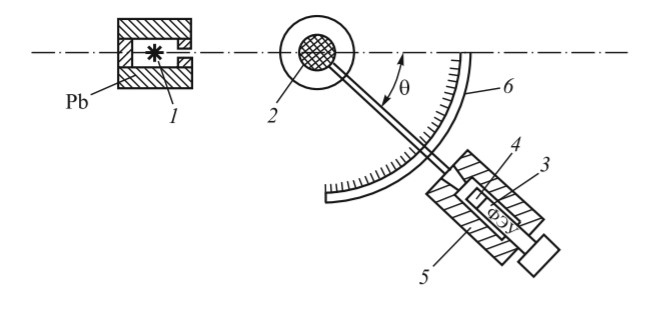
\includegraphics[width = \textwidth]{ust.jpg}
\caption{Экспериментальная установка}
\end{center}
\end{figure}

Кванты, испытавшие комптоновское рассеяние в мишени, регистрируются сцинтилляционным счетчиком, принцип работы которого рассмотрен в работе 5.3. Счетчик состоит из фотоэлектронного умножителя 3 (далее ФЭУ) и сцинтиллятора $4^{*}$ ). Сцинтиллятором служит кристалл NaI(Tl) цилиндрической формы диаметром 40 мм и высотой 40 мм, его выходное окно находится в оптическом контакте с фотокатодом ФЭУ. Сигналы, возникающие на аноде ФЭУ, подаются на ЭВМ для амплитудного анализа. Кристалл и ФЭУ расположены в светонепроницаемом блоке, укрепленном на горизонтальной штанге. Штанга вместе с этим блоком может вращаться относительно мишени, угол поворота отсчитывается по лимбу $6$.

\section{Используемое оборудование}

\begin{enumerate}
    \item компьютер;
    \item источник излучения;
    \item графитовая мишень;
    \item счётчик $\gamma$-квантов;
\end{enumerate}

\section{Результаты измерений и обработка данных}

Для обработки результатов используется формула $(2)$ с замененными энергиями квантов на $N(\theta)$.
\begin{equation}
\frac{1}{N(\theta)} - \frac{1}{N(0)} = A(1-\cos\theta)
\end{equation}

Сначала снимем спектр при $\theta = 0^0$:
\begin{figure}[h]
\begin{center}
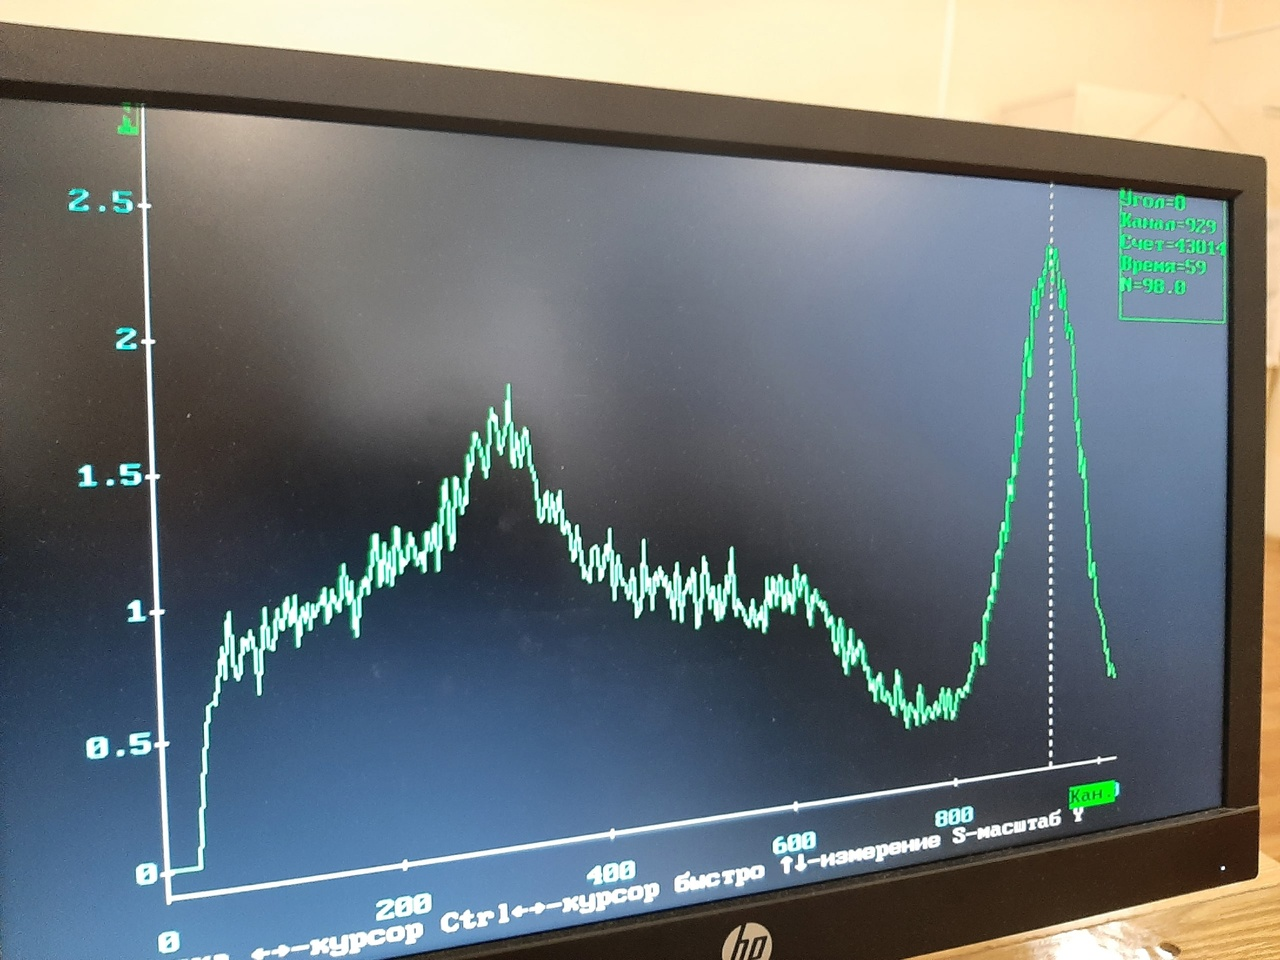
\includegraphics[width = 0.8\textwidth]{0.jpg}
\caption{$\theta = 0^0$}
\end{center}
\end{figure}

Далее устанавливая счётчик под разными углами, снимем амплитудные спектры при $\theta = 0\div120^0$.

\newpage

\begin{figure}[h]
\begin{minipage}[h]{0.3\linewidth}
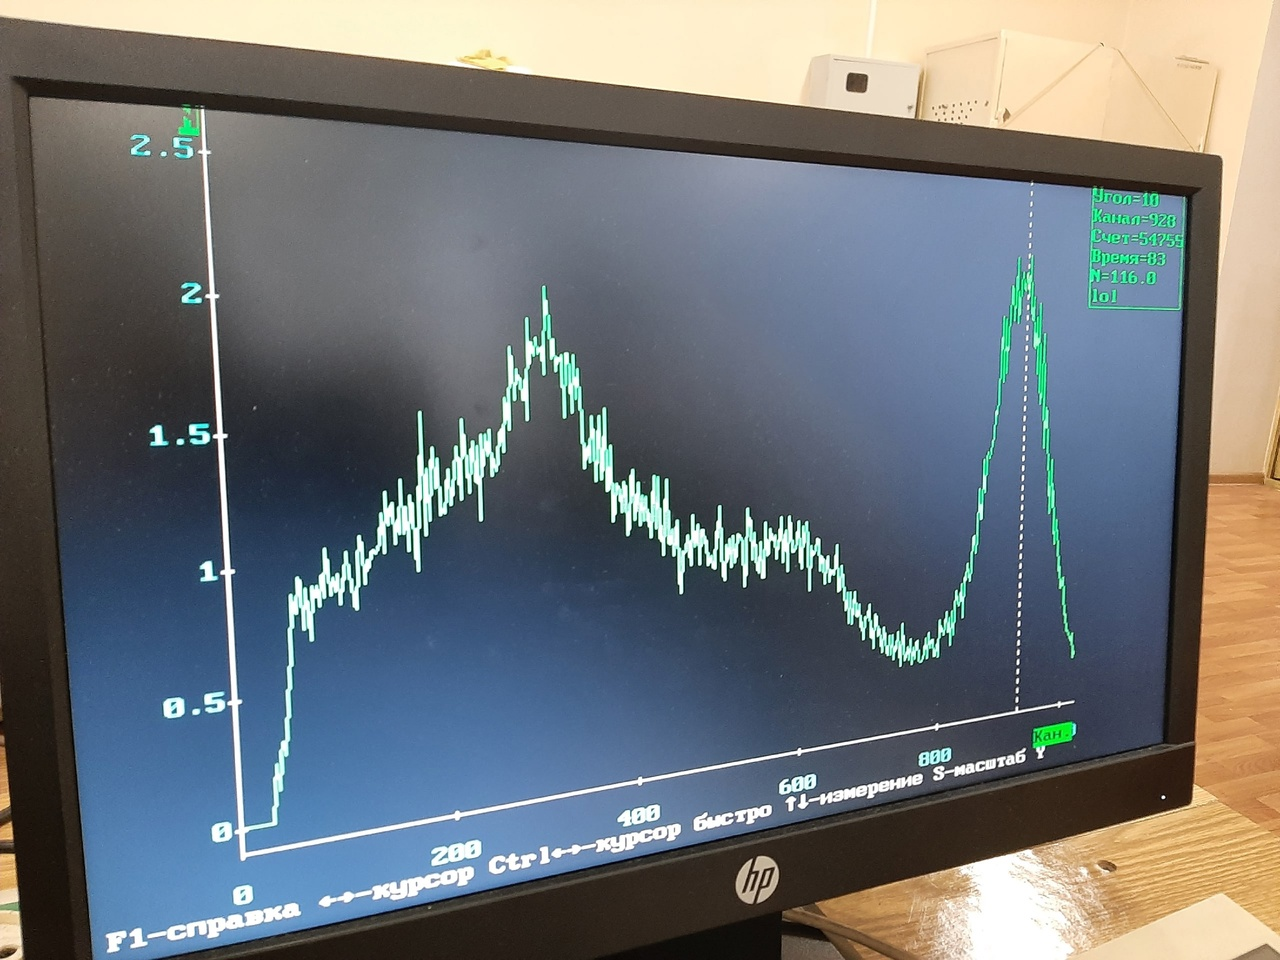
\includegraphics[width = 1\linewidth]{10.jpg}
\caption{$\theta = 10^0$}
\end{minipage}
\hfill
\begin{minipage}[h]{0.3\linewidth}
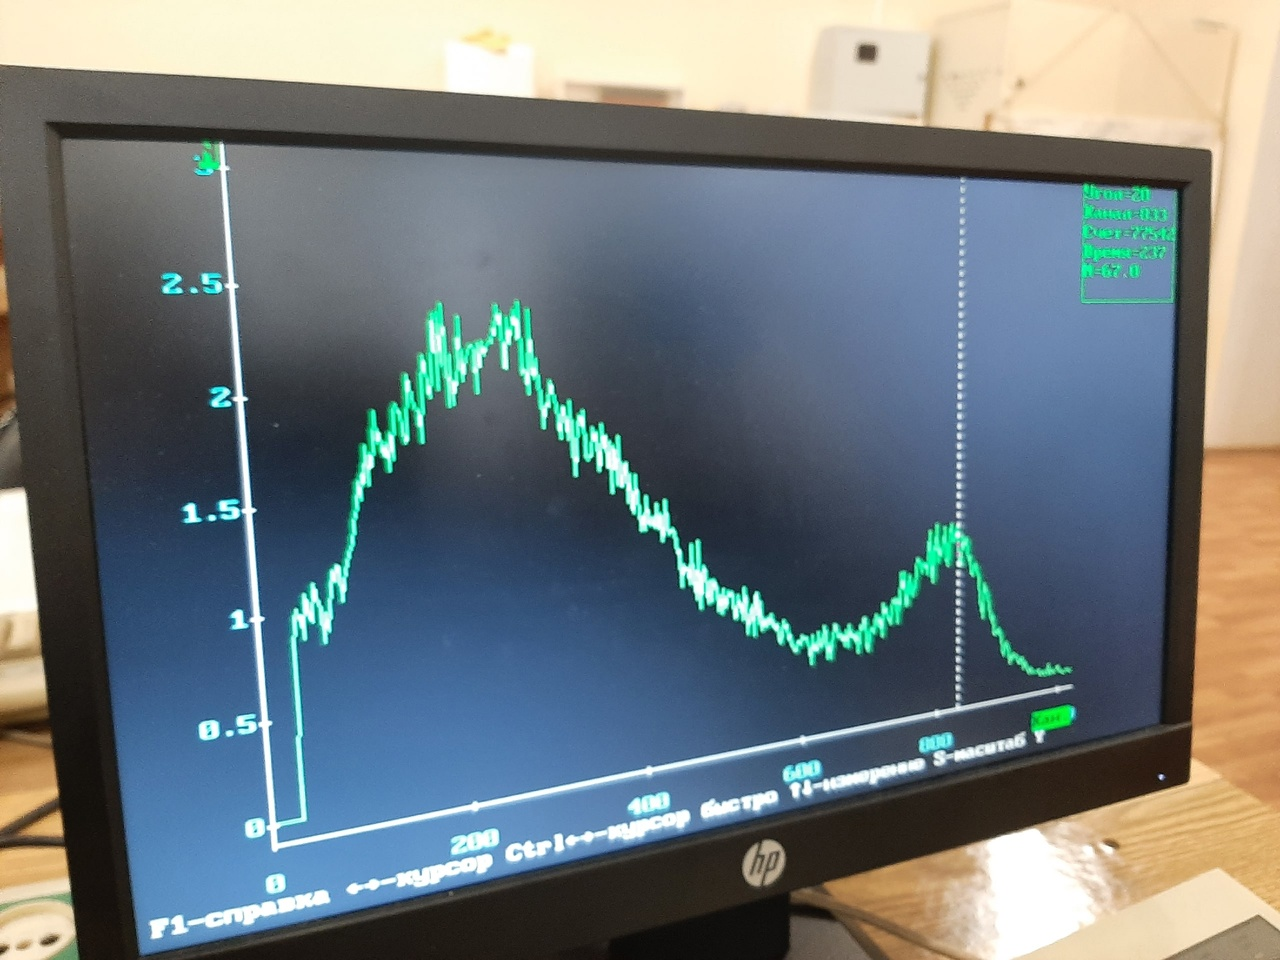
\includegraphics[width = 1\linewidth]{20.jpg}
\caption{$\theta = 20^0$}
\end{minipage}
\hfill
\begin{minipage}[h]{0.3\linewidth}
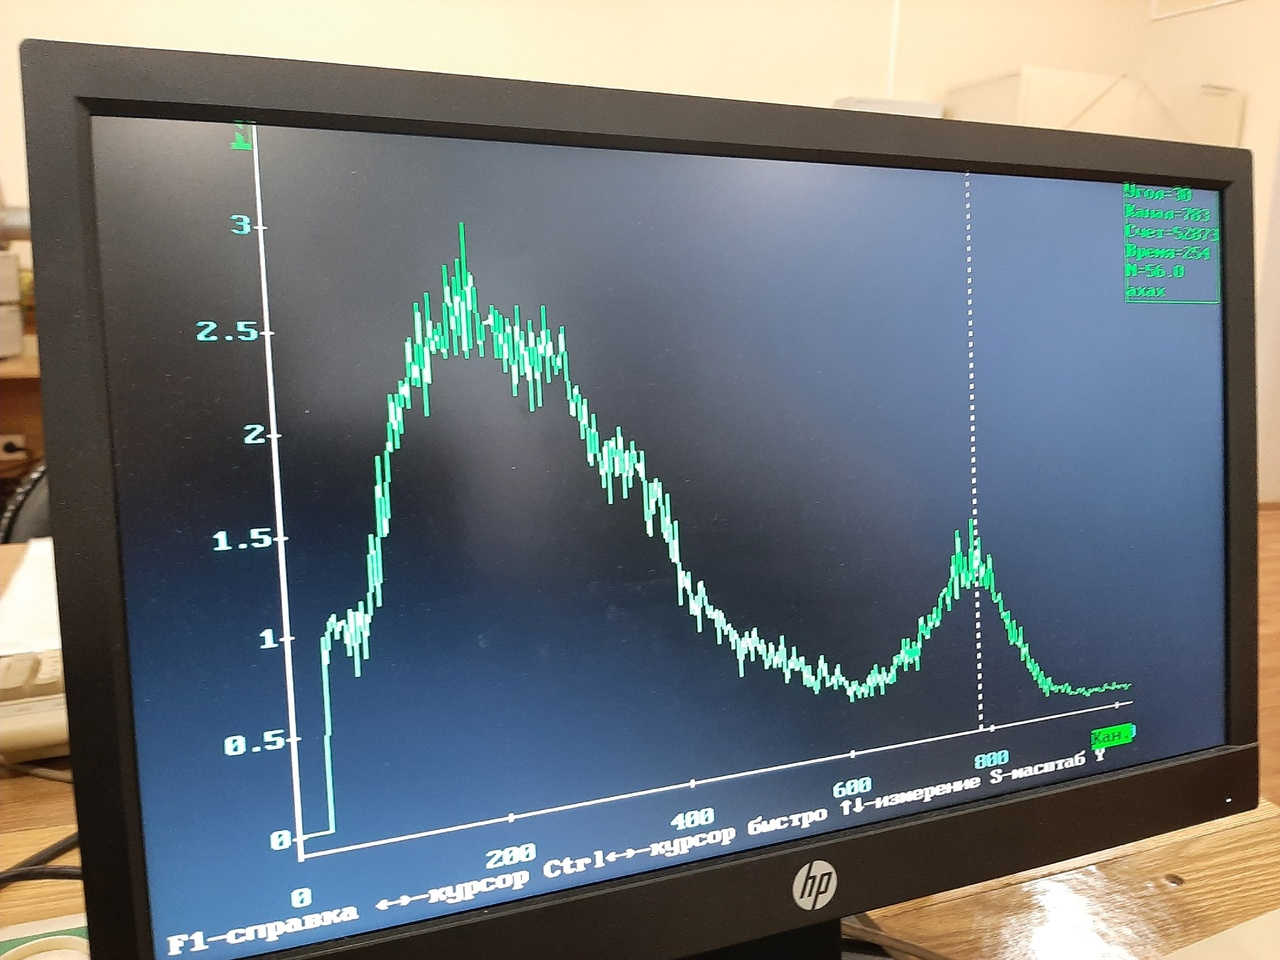
\includegraphics[width = 1\linewidth]{30.jpg}
\caption{$\theta = 30^0$}
\end{minipage}
\end{figure}
\begin{figure}[h]
\begin{minipage}[h]{0.3\linewidth}
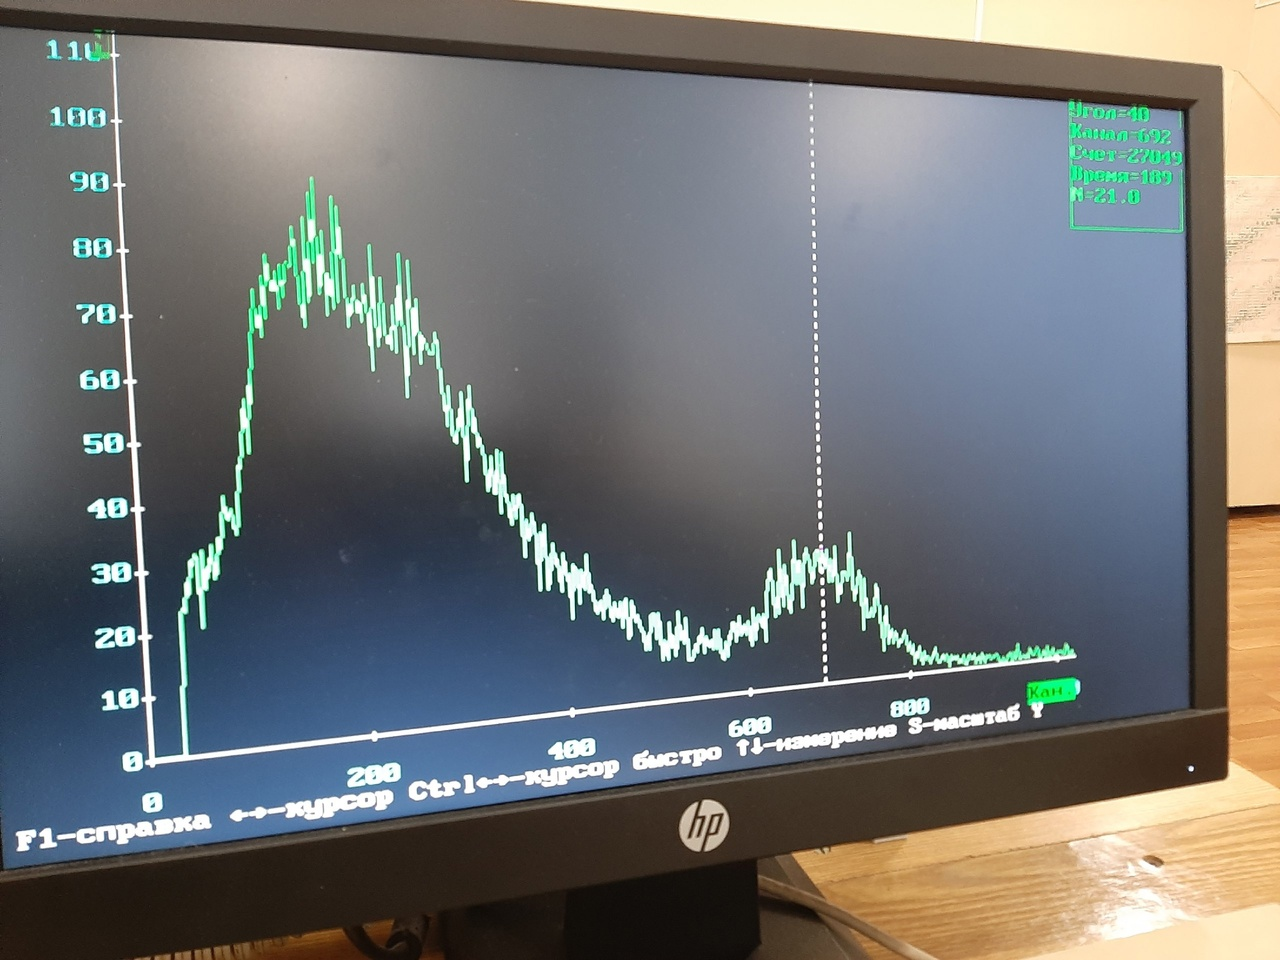
\includegraphics[width = 1\linewidth]{40.jpg}
\caption{$\theta = 40^0$}
\end{minipage}
\hfill
\begin{minipage}[h]{0.3\linewidth}
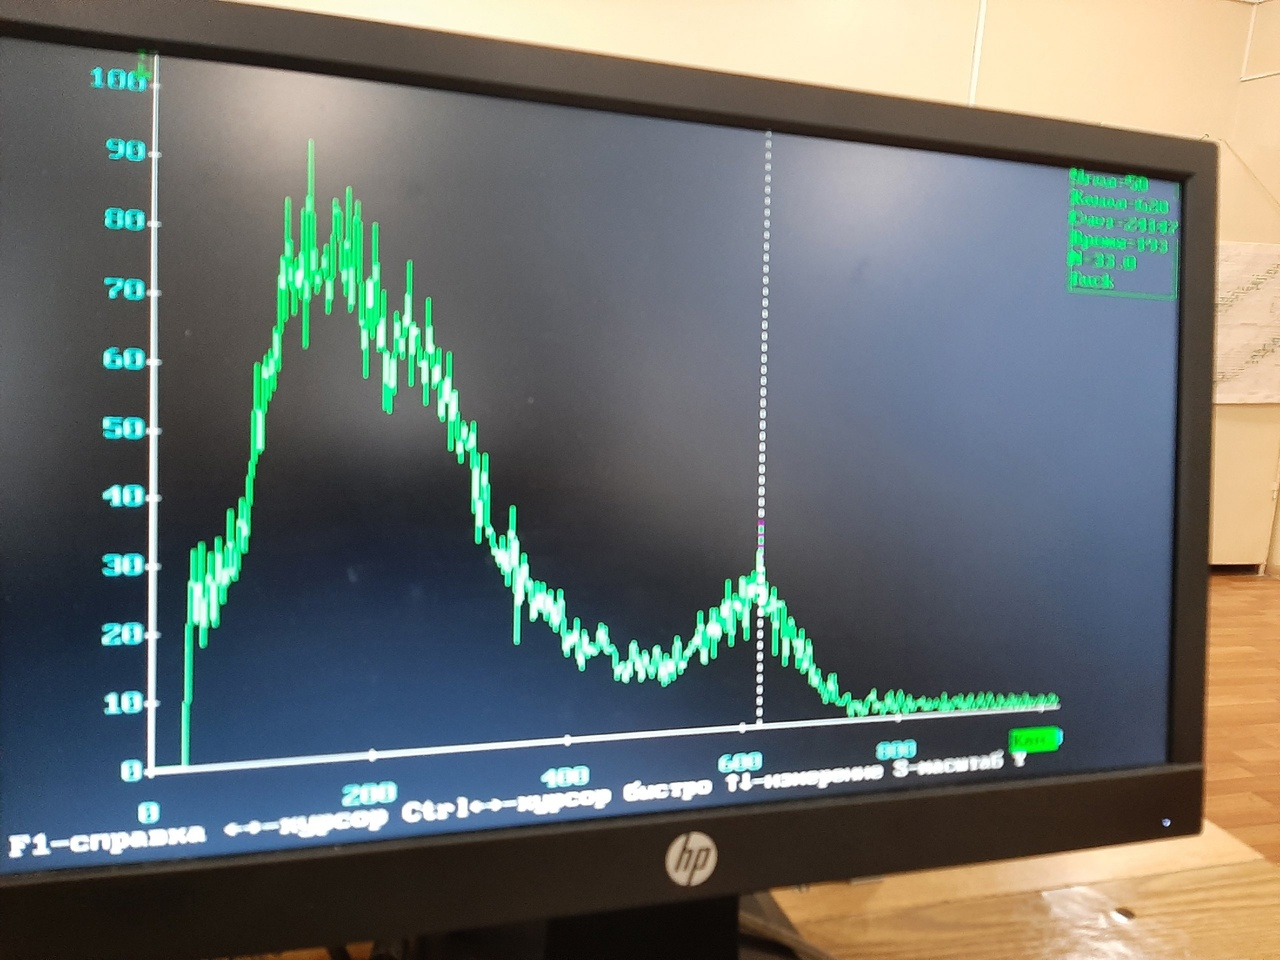
\includegraphics[width = 1\linewidth]{50.jpg}
\caption{$\theta = 50^0$}
\end{minipage}
\hfill
\begin{minipage}[h]{0.3\linewidth}
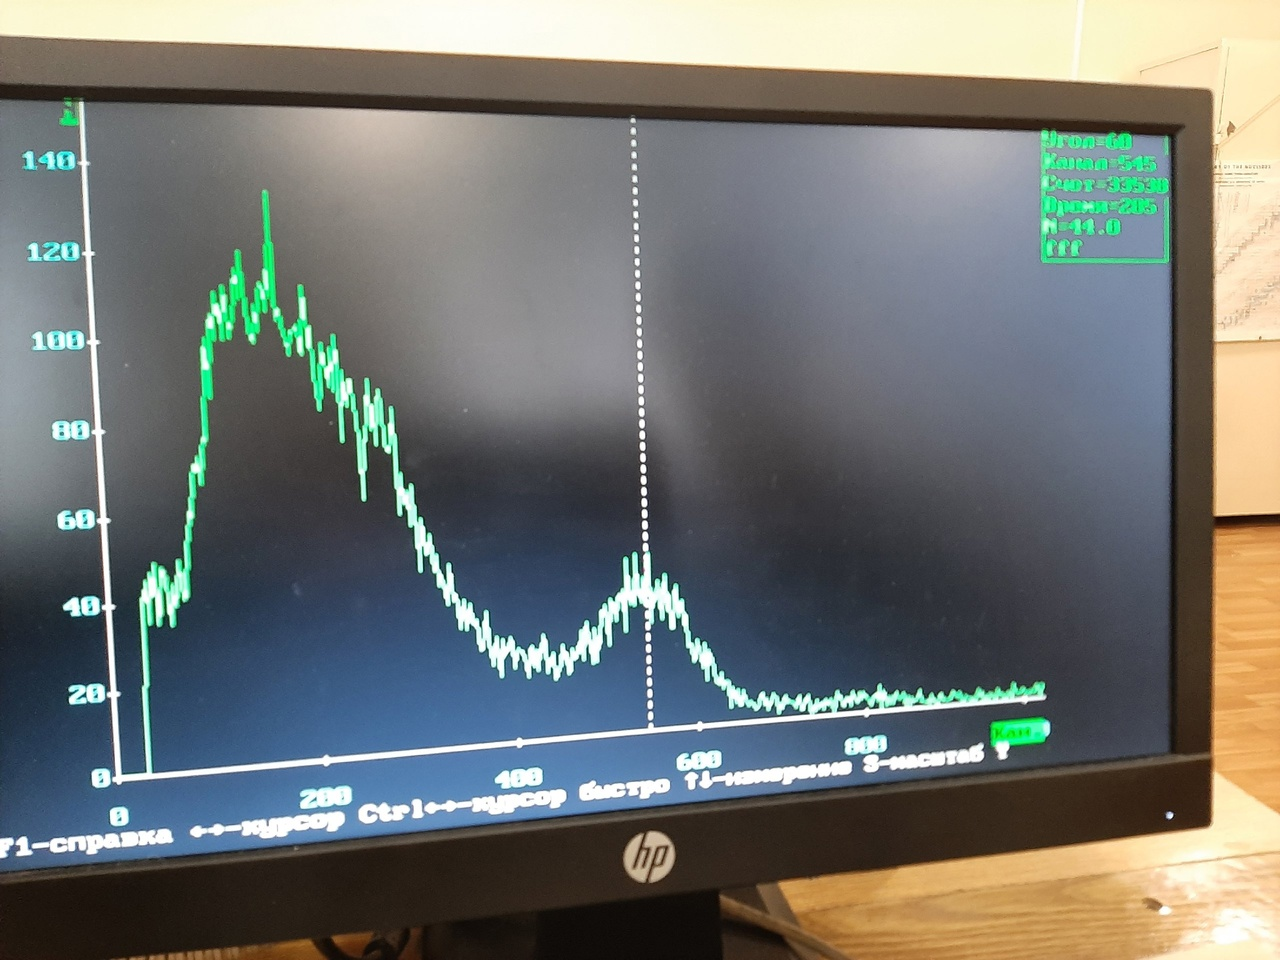
\includegraphics[width = 1\linewidth]{60.jpg}
\caption{$\theta = 60^0$}
\end{minipage}
\end{figure}
\begin{figure}[h]
\begin{minipage}[h]{0.3\linewidth}
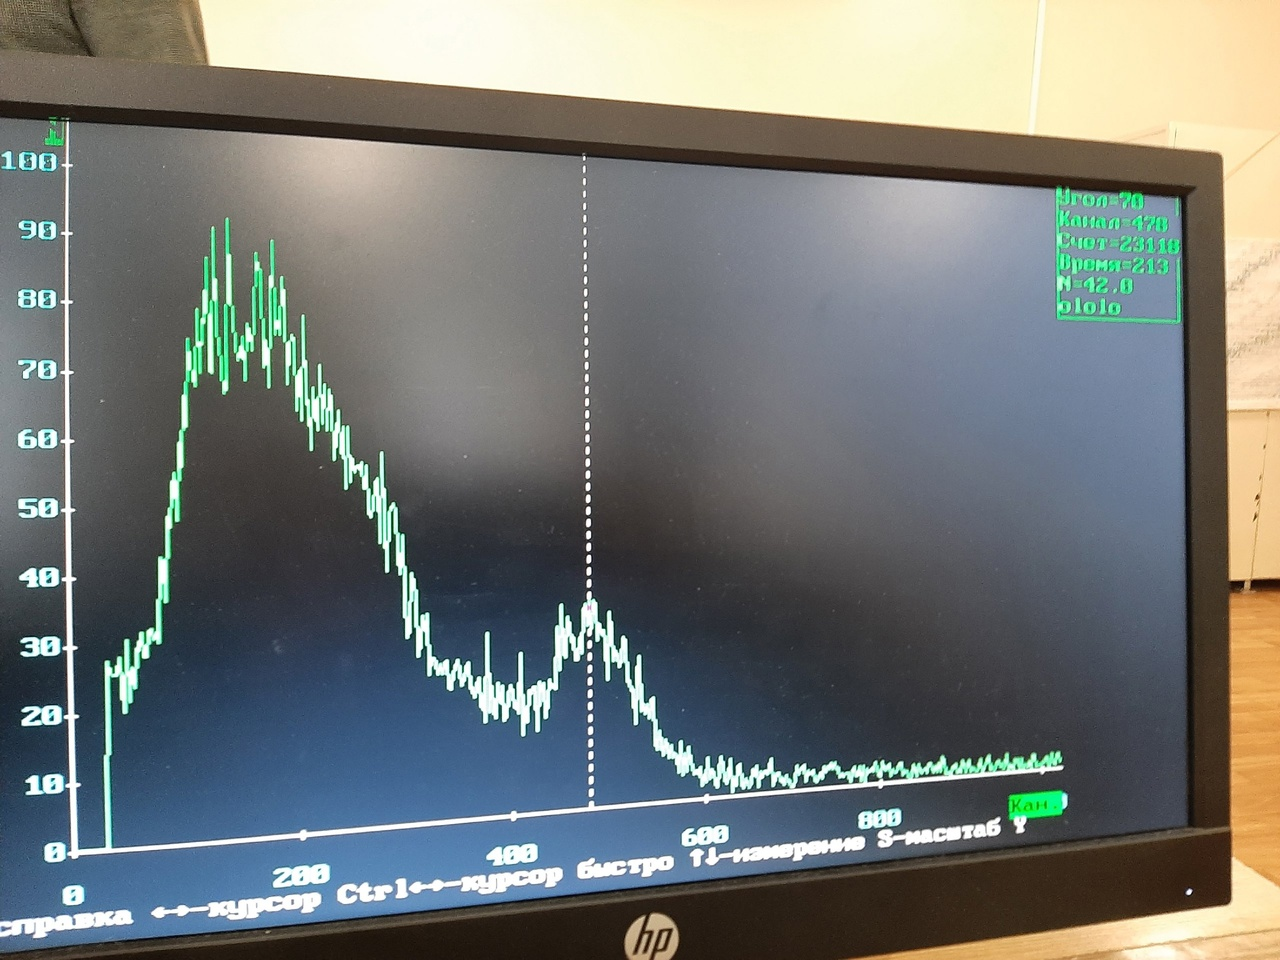
\includegraphics[width = 1\linewidth]{70.jpg}
\caption{$\theta = 70^0$}
\end{minipage}
\hfill
\begin{minipage}[h]{0.3\linewidth}
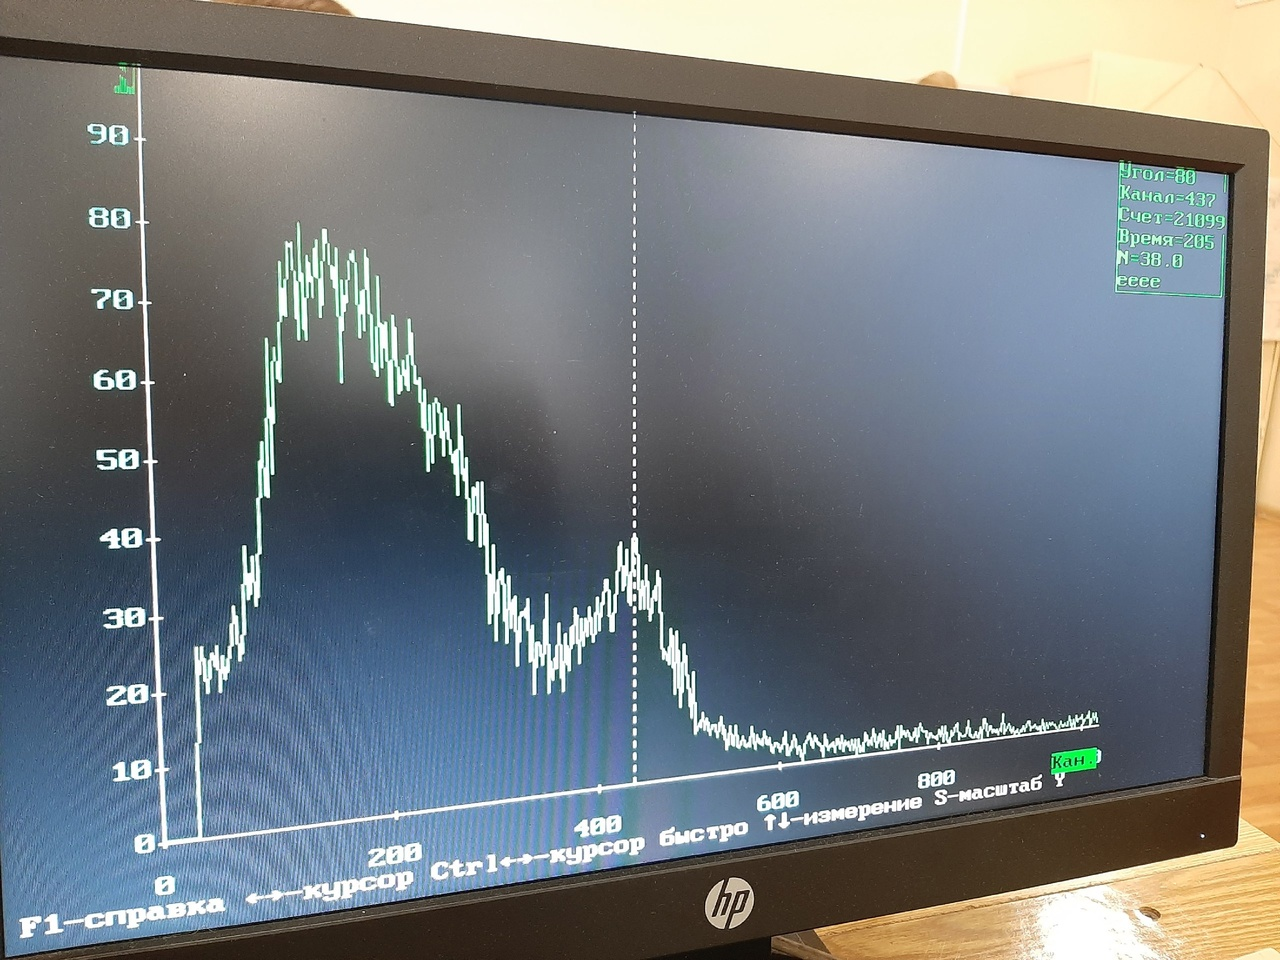
\includegraphics[width = 1\linewidth]{80.jpg}
\caption{$\theta = 80^0$}
\end{minipage}
\hfill
\begin{minipage}[h]{0.3\linewidth}
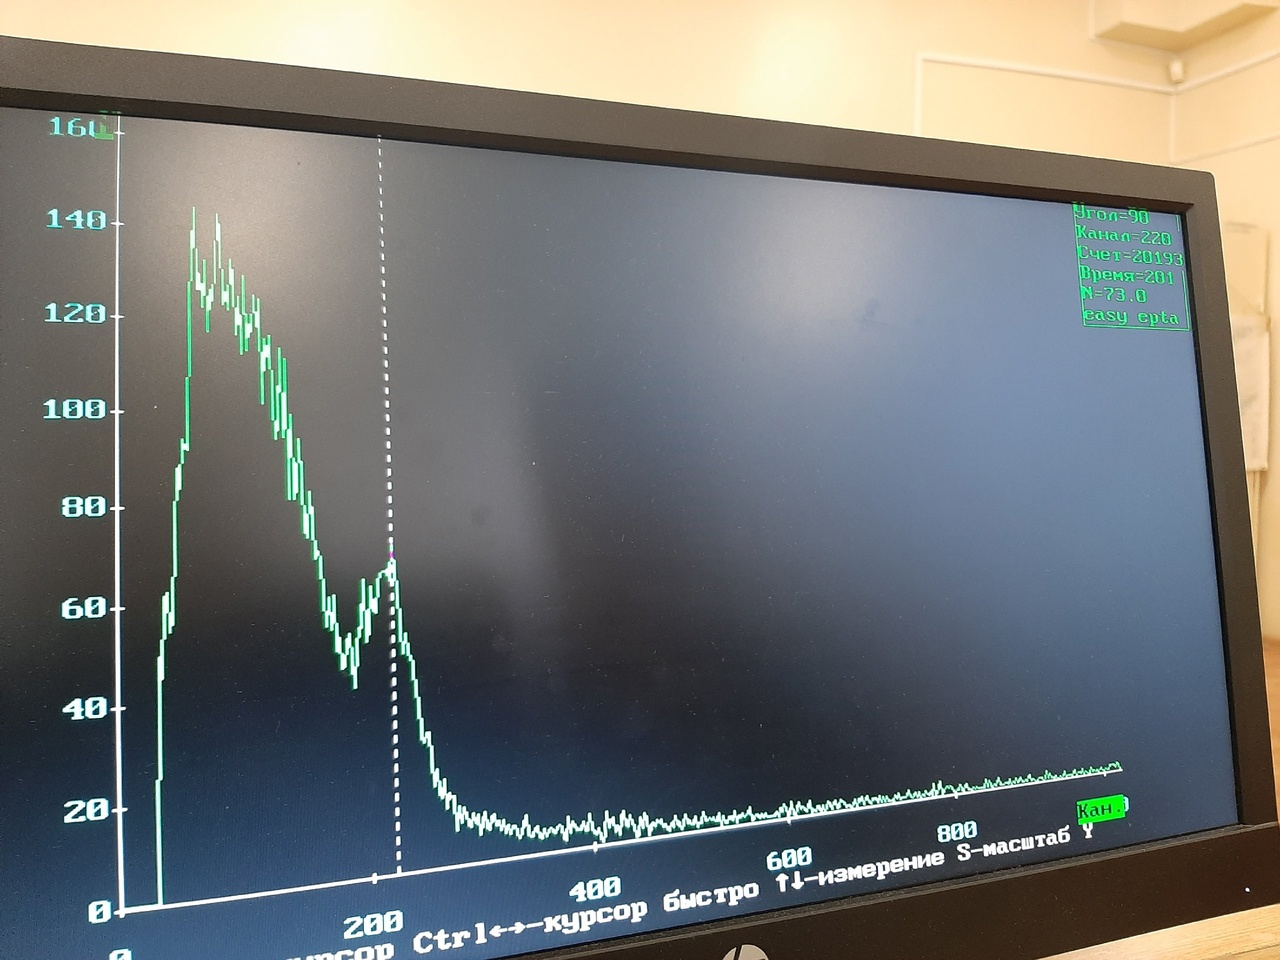
\includegraphics[width = 1\linewidth]{90.jpg}
\caption{$\theta = 90^0$}
\end{minipage}
\end{figure}
\begin{figure}[h]
\begin{minipage}[h]{0.3\linewidth}
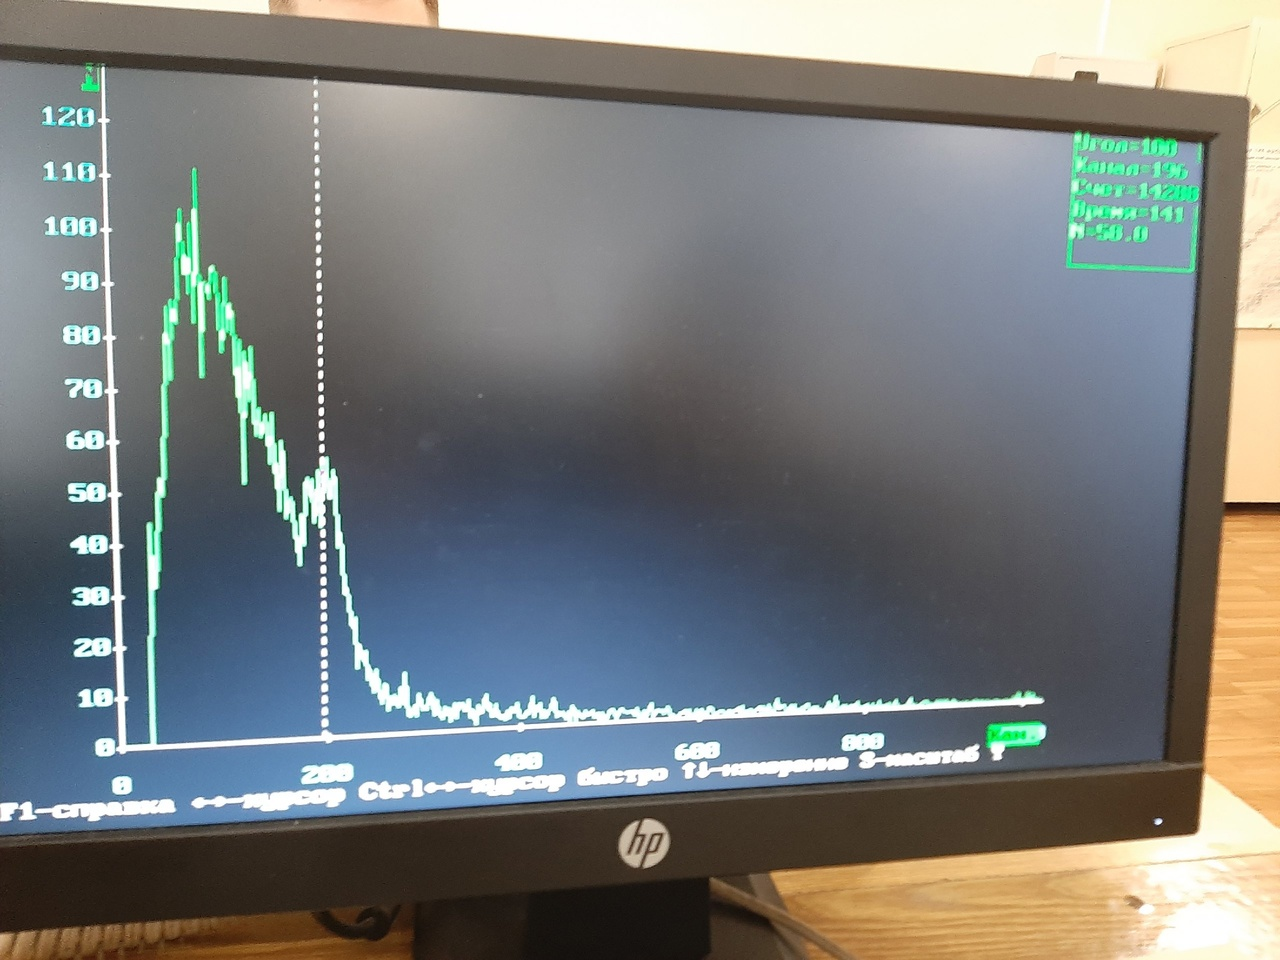
\includegraphics[width = 1\linewidth]{100.jpg}
\caption{$\theta = 100^0$}
\end{minipage}
\hfill
\begin{minipage}[h]{0.3\linewidth}
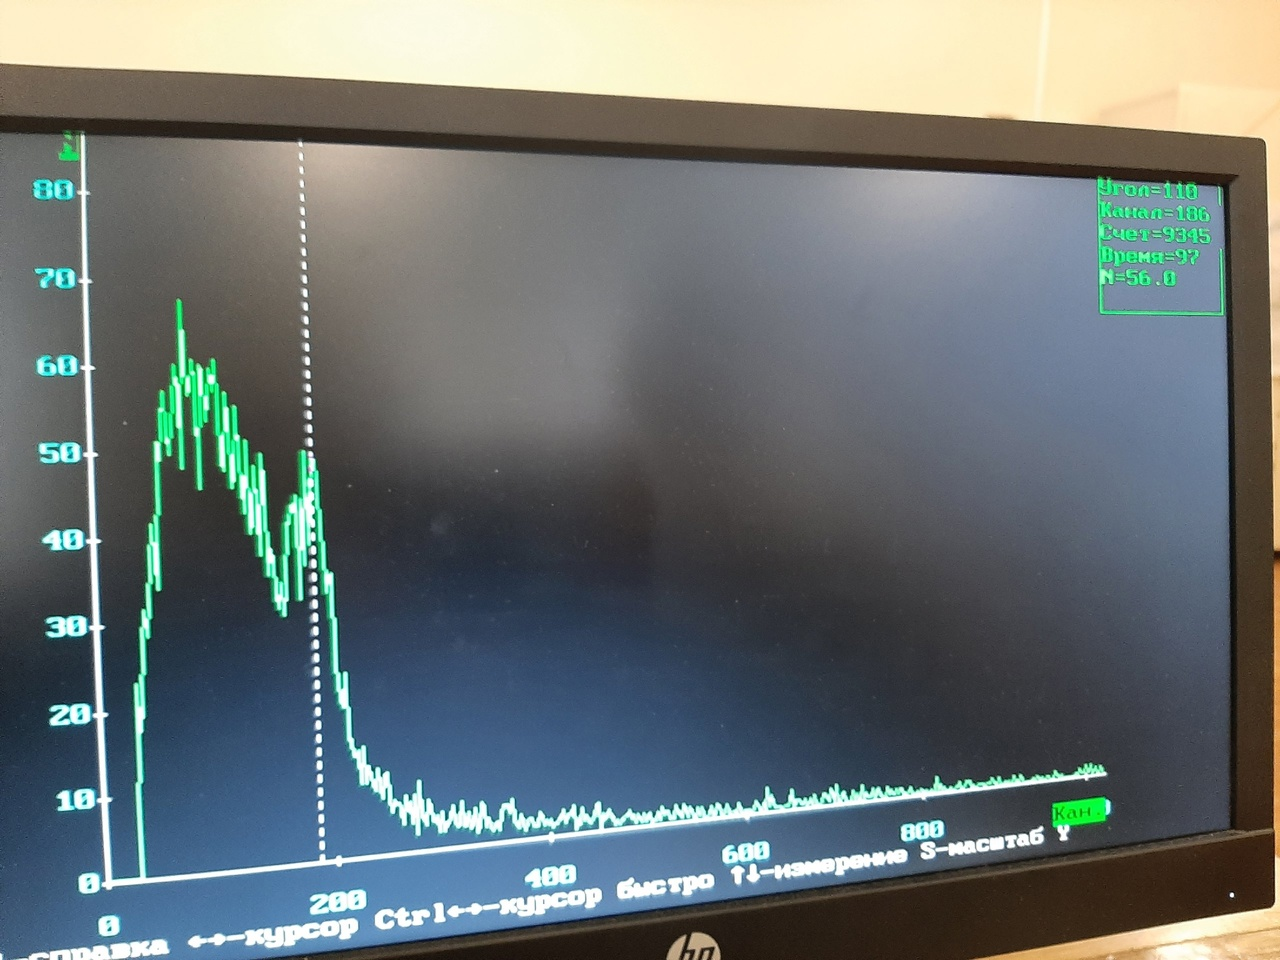
\includegraphics[width = 1\linewidth]{110.jpg}
\caption{$\theta = 110^0$}
\end{minipage}
\hfill
\begin{minipage}[h]{0.3\linewidth}
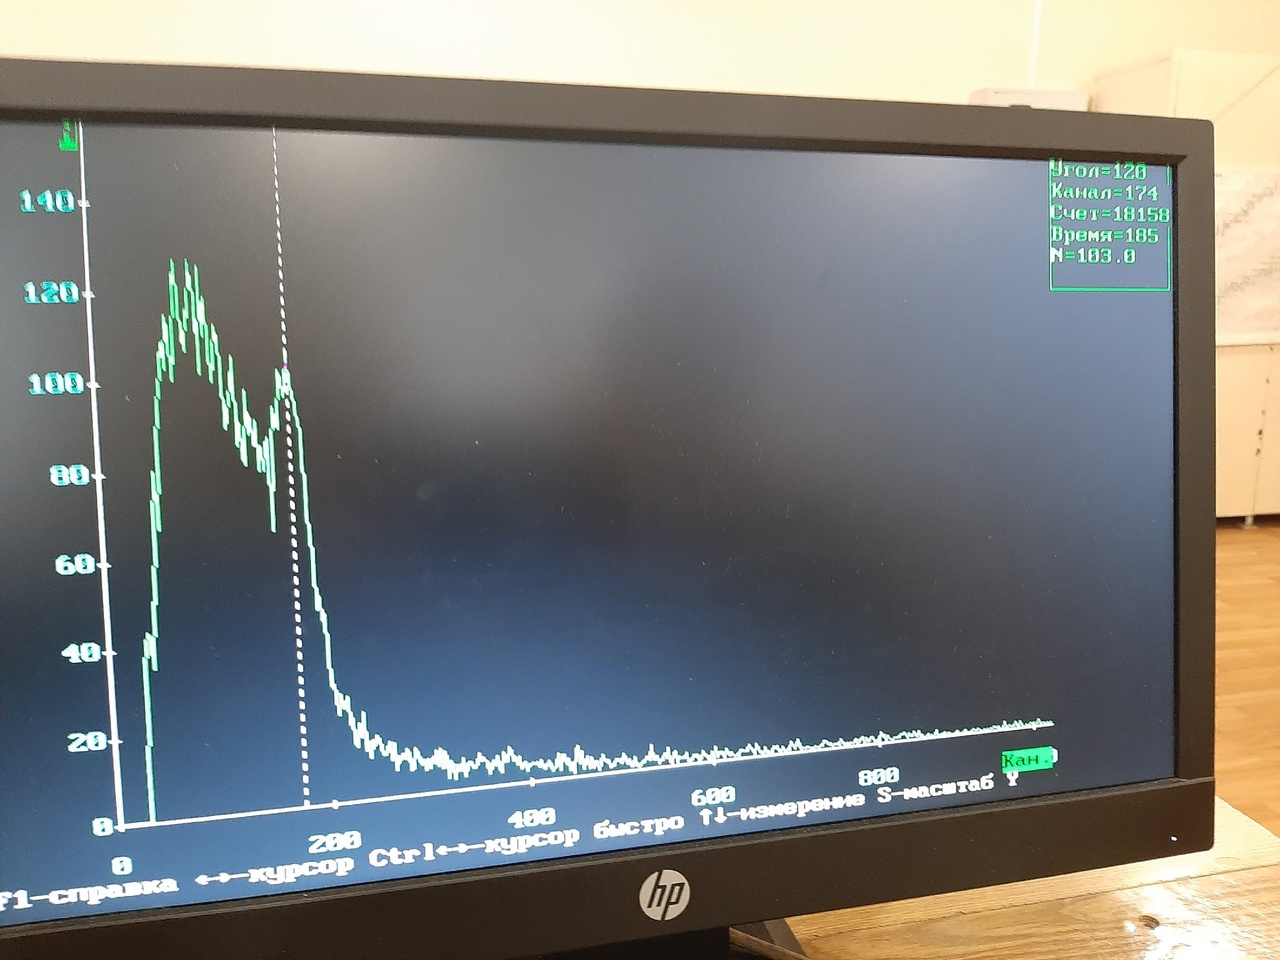
\includegraphics[width = 1\linewidth]{120.jpg}
\caption{$\theta = 120^0$}
\end{minipage}
\end{figure}

\newpage

По полученным спектрам определим положения фотопиков для каждого значения угла. Результаты представлены на рис.~\ref{tab:all}.

\begin{figure}[h]
\begin{center}
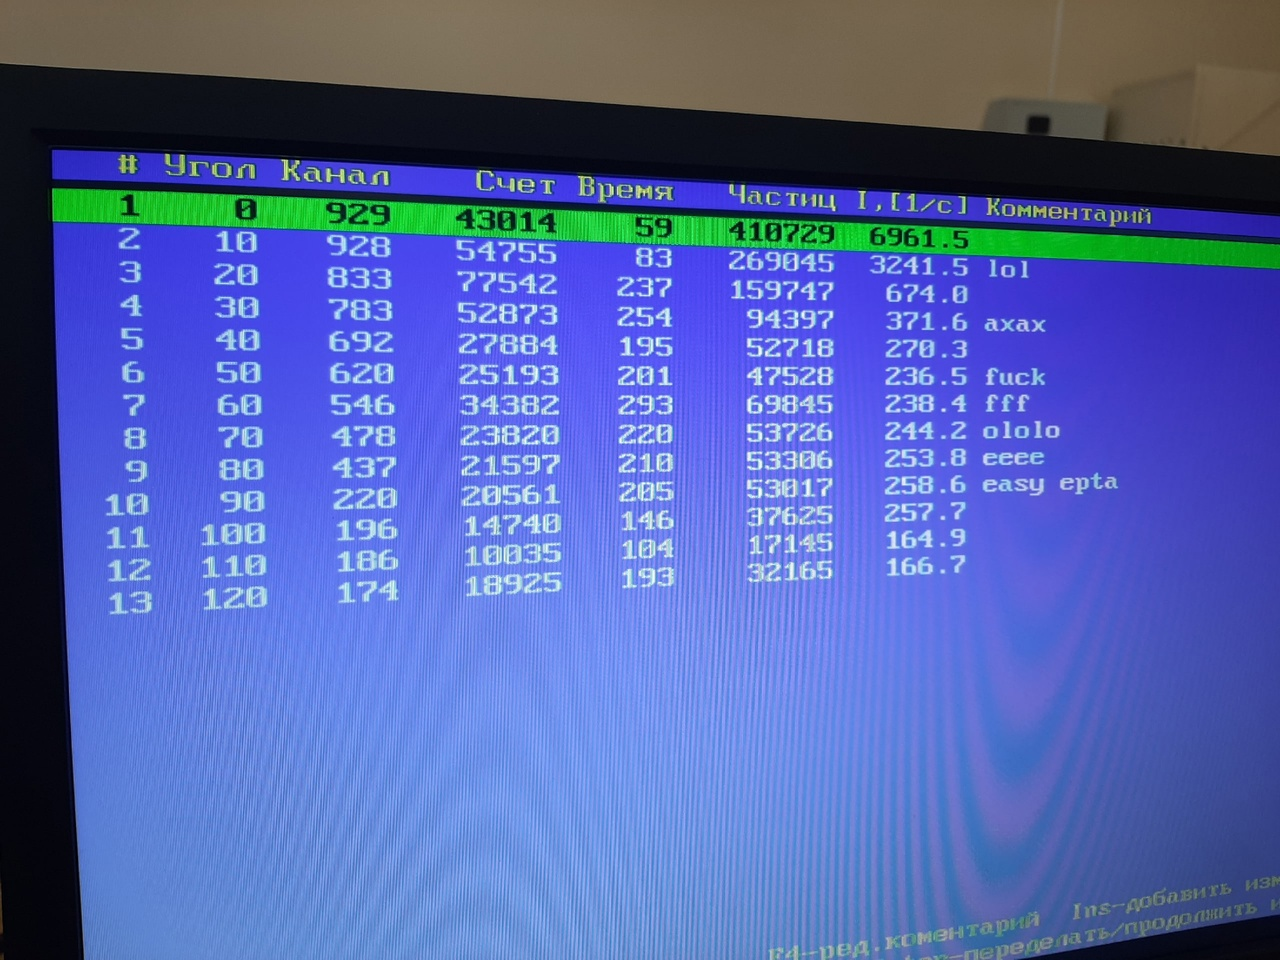
\includegraphics[width = 0.8\textwidth]{tab.jpg}
\caption{Результаты измерений}
\label{tab:all}
\end{center}
\end{figure}

По этим данным, использую $(3)$, построим график на рис.~\ref{fig:plot}.

\begin{figure}[h]
\begin{center}
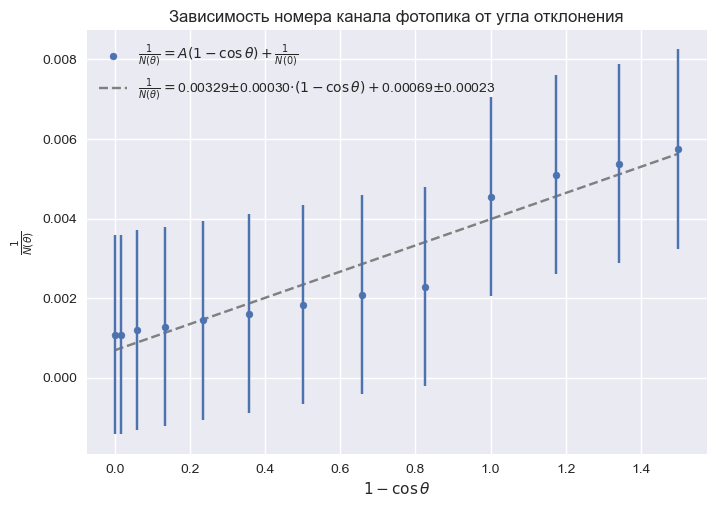
\includegraphics[width = \textwidth]{plot.png}
\caption{Зависимость $1/N(\theta)$ от $1 - \cos{\theta}$}
\label{fig:plot}
\end{center}
\end{figure}

По графику определим $N(0) = 1449\pm483$, $N(90) = 250\pm33$. Теперь посчитаем энергию покоя частицы из формулы $(2)$, где $E_{\gamma} = 662~кэВ$ --- энергия $\gamma$-квантов $Cs^{137}$. В итоге получаем:
\begin{equation}
mc^2 = E_{\gamma} \frac{N(90)}{N(0) - N(90)} = 138\pm58~кэВ.
\end{equation}

\newpage

\section{Обсуждение результатов и выводы}

По результатам работы, исследовали эффект Комптона на графитовом образце с помощью сцинтилляционного спектрометра. Выяснили зависимость  энергии рассеянного $\gamma$-кванта от угла рассеяния, а также определили по порядку величины энергию покоя электрона. Полученное значение:
\begin{equation}
\boxed{mc^2 = 138\pm58~кэВ}
\end{equation}
Это значение существенно отличается от табличного для энергии покоя электрона, что может быть связано как с неточным проведением эксперимента, так и с тем, что электрон  в составе атома не является свободным, поэтому исходная формула $(2)$ не является достаточно точной в данном случае.

\end{document}
